\documentclass[11pt]{article}
\usepackage{acl2016}
\usepackage{times}

\usepackage{url}
\usepackage{latexsym}
\usepackage{booktabs}
\usepackage{multirow}
\usepackage{graphicx}
\usepackage{paralist}
\usepackage{mathtools}
\usepackage{dingbat}
\usepackage{subcaption}
\usepackage{balance}
\usepackage{gensymb}
\usepackage{marginnote}
\usepackage{adjustbox}
\usepackage{url}

% \makeatletter
% \newcommand{\@BIBLABEL}{\@emptybiblabel}
% \newcommand{\@emptybiblabel}[1]{}
% \makeatother
% \usepackage{hyperref}

% \sloppy

\aclfinalcopy % Uncomment this line for the final submission
\def\aclpaperid{30} %  Enter the acl Paper ID here


\usepackage{color}
\newcommand{\todo}[1]{}
\renewcommand{\todo}[1]{{\color{red} TODO: {#1}}}

% \renewcommand{\baselinestretch}{0.95}

%\setlength\titlebox{5cm}

% You can expand the titlebox if you need extra space
% to show all the authors. Please do not make the titlebox
% smaller than 5cm (the original size); we will check this
% in the camera-ready version and ask you to change it back.

\title{Robust Co-occurrence Quantification for Lexical Distributional Semantics}

\author{Dmitrijs Milajevs\qquad{}Mehrnoosh Sadrzadeh\qquad{}Matthew Purver\\
  Queen Mary University of London\\
  London, UK\\
  {\tt \{d.milajevs,m.sadrzadeh,m.purver\}@qmul.ac.uk}
}
\date{}

\newcommand{\BASEURL}{http://example.org}
% \newcommand{\BASEURL}{https://bitbucket.org/dimazest/phd-buildout/raw/tip/notebooks/downloads/compdistmeaning}
\newcommand{\dataurl}[1]{\href{\BASEURL/#1}{\nolinkurl{#1}}}

\newcommand{\p}{\textsuperscript{\textasteriskcentered}}
\newcommand{\pw}{\textsuperscript{\dag}}

\newcommand{\pp}{\textsuperscript\dag}
\newcommand{\ppp}{\textsuperscript\ddag}
\newcommand{\np}{\phantom{\textsuperscript\textasteriskcentered}}

\begin{document}

\def\PMI/{$\operatorname{1PMI}$}
\def\SPMI/{$\operatorname{1SPMI}$}
\def\CPMI/{$\operatorname{1CPMI}$}
\def\SCPMI/{$\operatorname{1SCPMI}$}

\def\NPMI/{$\operatorname{nPMI}$}
\def\NSPMI/{$\operatorname{nSPMI}$}
\def\NCPMI/{$\operatorname{nCPMI}$}
\def\NSCPMI/{$\operatorname{nSCPMI}$}

\def\logNPMI/{$\operatorname{lognPMI}$}
\def\logNSPMI/{$\operatorname{lognSPMI}$}
\def\logNCPMI/{$\operatorname{lognCPMI}$}
\def\logNSCPMI/{$\operatorname{lognSCPMI}$}

\maketitle
\begin{abstract}
Previous optimisations of parameters affecting the word-context association measure used in distributional vector space models have focused either on high-dimensional vectors with hundreds of thousands of dimensions, or dense vectors with dimensionality of a few hundreds; but dimensionality of a few thousands is often applied in compositional tasks as it is still computationally feasible and does not require the dimensionality reduction step. We present a systematic study of the interaction of the parameters of the association measure and vector dimensionality, and derive parameter selection heuristics that achieve performance across word similarity and relevance datasets competitive with the results previously reported in the literature achieved by highly dimensional or dense models.
\end{abstract}

\section{Introduction}
\label{sec:introduction}

Words that occur in similar context have similar meaning \cite{harris1954distributional}. Thus the meaning of a word can be modeled by counting its co-occurrence with neighboring words in a corpus. Distributional models of meaning represent co-occurrence information in a vector space, where the dimensions are the neighboring words and the values are co-occurrence counts. Successful models need to be able to discriminate co-occurrence information, as not all co-occurrence counts are equally useful, for instance, the co-occurrence with the article \textit{the} is less informative than with the noun \textit{existence}. The discrimination is usually achieved by weighting of co-occurrence counts. Another fundamental question in vector space design is the vector space dimensionality and what neighbor words should correspond to them.

\newcite{TACL570} propose optimisations for co-occurrence-based distributional models, using parameters adopted from predictive models \cite{mikolov2013efficient}: \emph{shifting} and \emph{context distribution smoothing}. Their experiments and thus their parameter  recommendations use high-dimensional vector spaces with word vector dimensionality of almost \textbf{200K}, and many recent state-of-the-art results in lexical distributional semantics have been obtained using vectors with similarly high dimensionality  \cite{baroni-dinu-kruszewski:2014:P14-1,kiela-clark:2014:CVSC,lapesa2014large}.

In contrast, much work on \emph{compositional} distributional semantics employs vectors with much fewer dimensions: e.g.~\textbf{2K} \cite{Grefenstette:2011:ESC:2145432.2145580,kartsadrqpl2014,milajevs-EtAl:2014:EMNLP2014}, \textbf{3K} \cite{Dinu:2010:MDS:1870658.1870771,milajevs-purver:2014:CVSC} or \textbf{10K} \cite{polajnar-clark:2014:EACL,Baroni2010nouns}. The most common reason thereof is that these models  assign tensors to functional words. For a vector space $V$ with $k$ dimensions,  a tensor $V \otimes V \cdots \otimes V$ of rank $n$ has $k^n$ dimensions. Adjectives and intransitive verbs have tensors of rank 2, transitive verbs are of rank 3; for coordinators, the rank can go up to 7. Taking $k = \textbf{200K}$ already results in a highly intractable tensor of $\textbf{8} \times \textbf{10}^{\textbf{15}}$ dimensions for a transitive verb.

An alternative way of obtaining a vector space with few dimensions, usually with just 100--500, is the use of SVD as a part of Latent Semantic Analysis \cite{ARIS:ARIS1440380105} or another models such as SGNS \cite{mikolov2013efficient} and GloVe \cite{pennington2014glove}. However, these models take more time to instantiate in comparison to weighting of a co-occurrence matrix, bring more parameters to explore and produce vector spaces with uninterpretable dimensions (vector space dimension interpretation is used by some lexical models, for example, \newcite{McGregorEtAl15JAGI}, and the passage from formal semantics to tensor models relies on it \cite{DBLP:journals/corr/abs-1003-4394}). In this work we focus on vector spaces that directly weight a co-occurrence matrix and report results for SVD, GloVe and SGNS from the study of \newcite{TACL570} for comparison.

The mismatch of recent experiments with non-dense models in vector dimensionality between lexical and compositional tasks gives rise to a number of questions:
\begin{compactitem}
\item To what extent does model performance depend on vector dimensionality?
\item Do parameters influence 200K and 1K dimensional models similarly? Can the findings of \newcite{TACL570} be directly applied to models with a few thousand dimensions?
\item If not, can we derive suitable parameter selection heuristics which take account of dimensionality?
\end{compactitem}

To answer these questions, we perform a systematic study of distributional models with a rich set of parameters on SimLex-999  \cite{hill2014simlex}, a lexical \emph{similairty} dataset, and test selected models on MEN \cite{Bruni:2014:MDS:2655713.2655714}, a lexical \emph{relatedness} dataset. The reason for choosing these is that they are currently widely used and surpass datasets stemming from information retrieval, WordSim-353 \cite{2002:PSC:503104.503110}, and computational linguistics, RG65 \cite{Rubenstein:1965:CCS:365628.365657}, in quantity by having more entries and in quality by attention to evaluated relations.

\section{Parameters}
\label{sec:parameters}

\begin{figure*}
  \centering
    \centerline{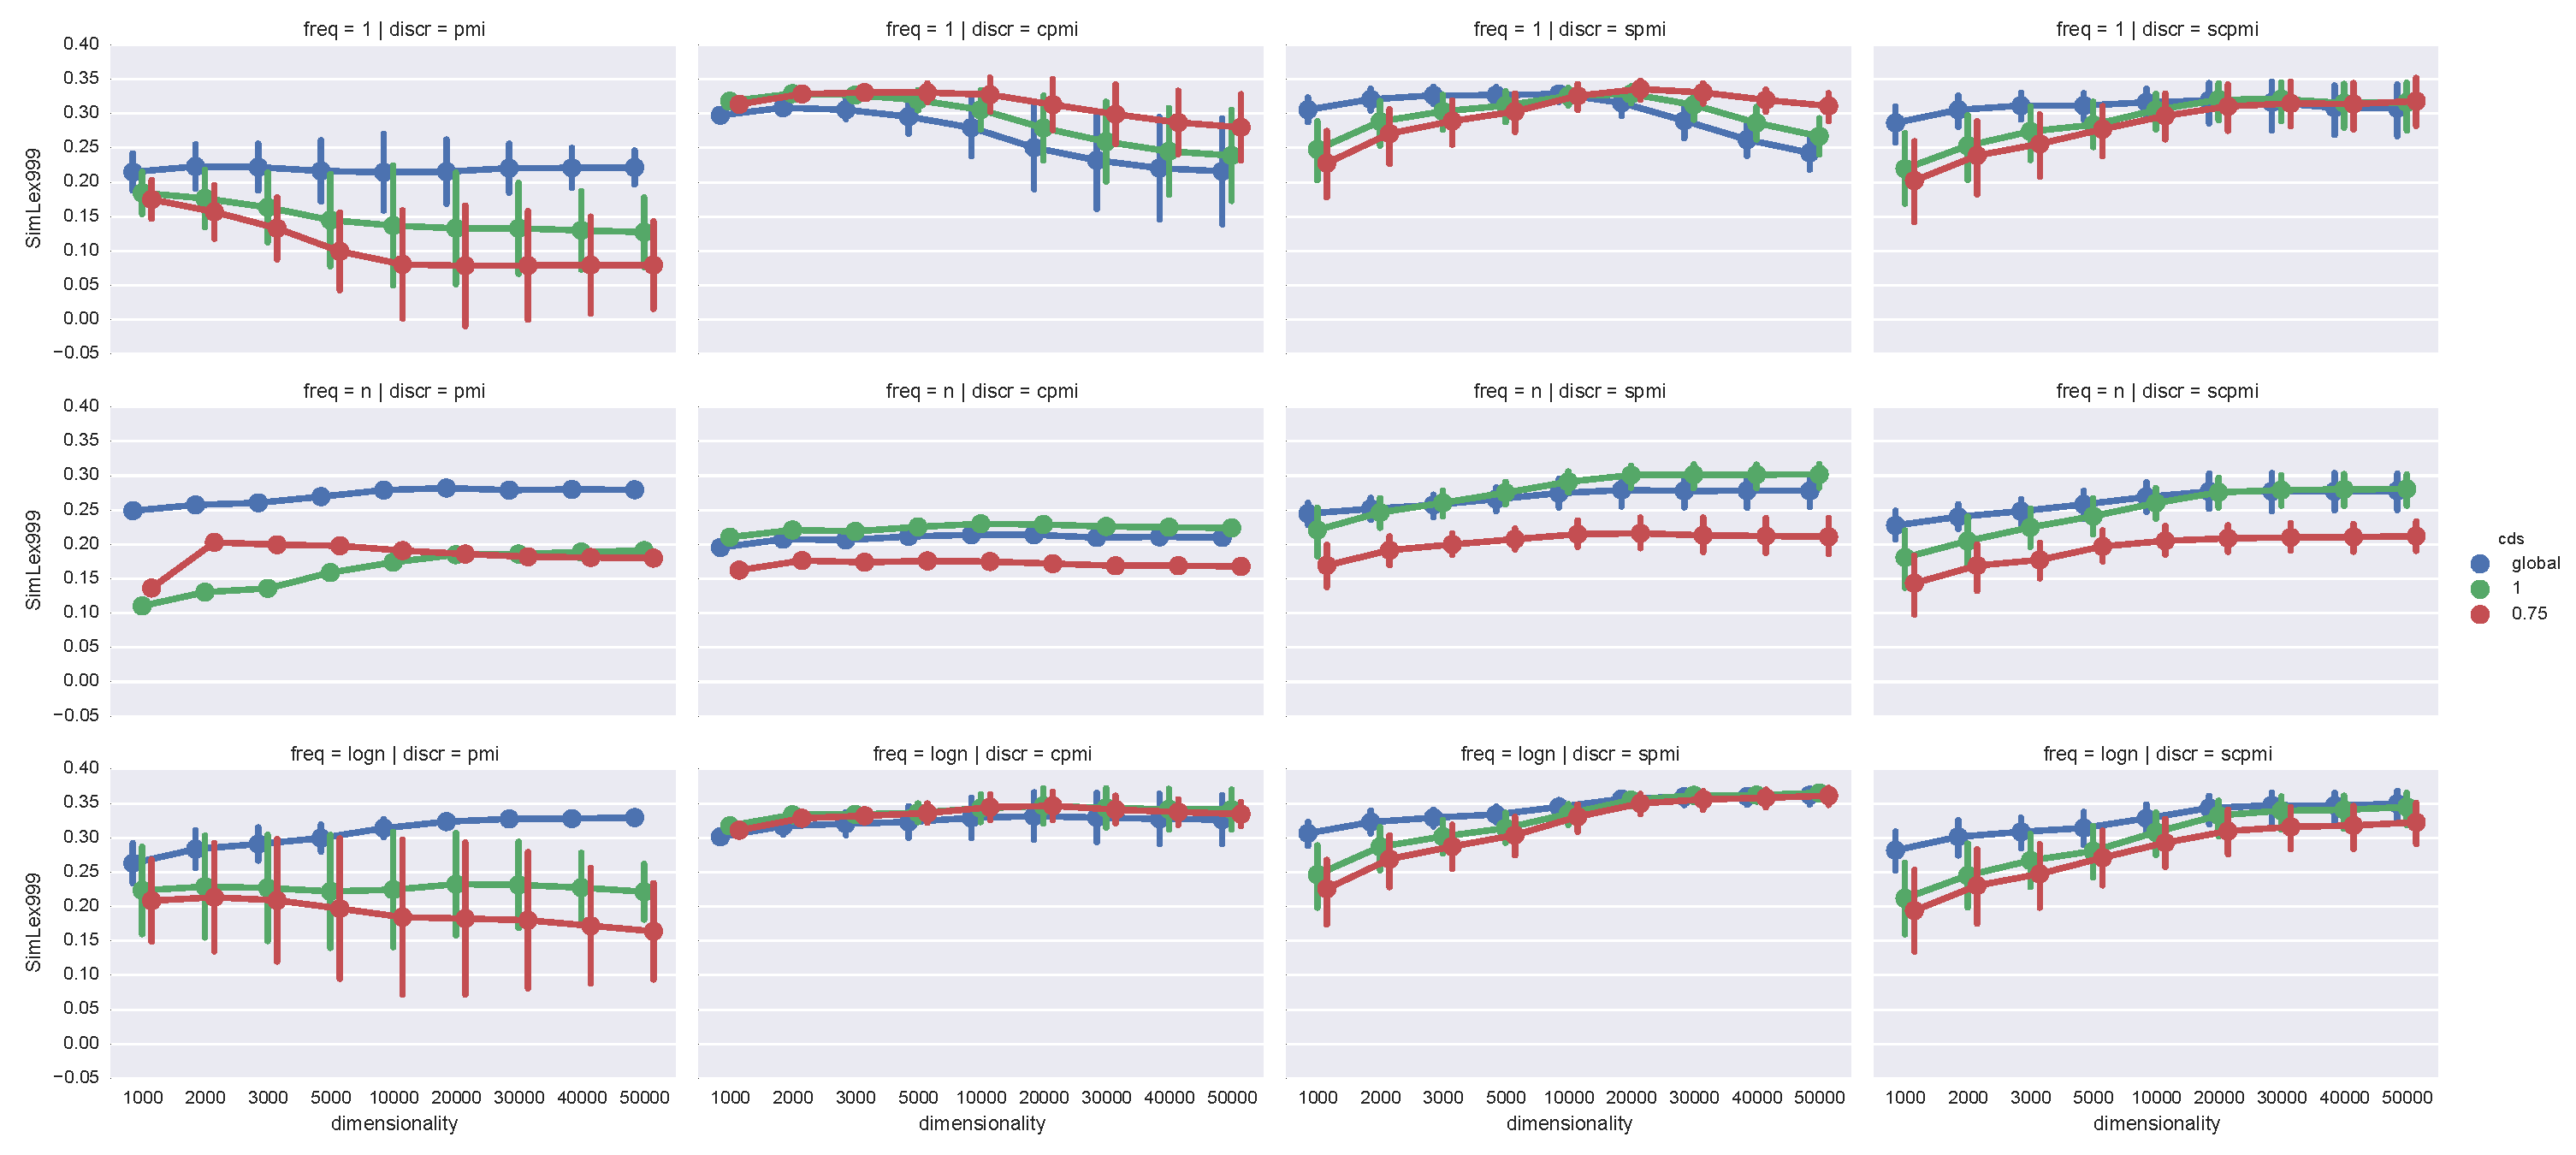
\includegraphics[width=1.11\textwidth]{supplement/figures/SimLex999-interaction-cds}}
    \caption{{\bf Effect of PMI variant (\texttt{discr}), smoothing (\texttt{cds}) and frequency weighting (\texttt{freq}) on SimLex-999.} Error bars correspond to a 95\% confidence interval as the value is estimated by aggregating over omitted parameters: \texttt{neg} and similarity.}
    \label{fig:interaction-cds}
\end{figure*}

%%% Local Variables:
%%% mode: latex
%%% TeX-master: "paper"
%%% End:


\subsection{PMI variants (\texttt{discr})}
\label{sec:pmi-variants}

Most co-occurrence weighting schemes in distributional semantics are based on \emph{point-wise mutual information} (PMI, see e.g.~\newcite{J90-1003}, \newcite{Turney:2010:FMV:1861751.1861756}, \newcite{NIPS2014_5477}):
%
\begin{equation}
  \label{eq:pmi}
  \operatorname{PMI}(x, y) = \log\frac{P(x,y)}{P(x)P(y)}
\end{equation}
%
As commonly done, we replace the infinite PMI values,\footnotemark{} which arise when $P(x, y) = 0$, with zeroes and use PMI hereafter to refer to a weighting with this fix.

\footnotetext{We assume that the probability of a single token is always greater than zero as it appears in the corpus at least once.}

An alternative solution is to increment the probability ratio by 1; we refer to this as \textit{compressed PMI} (CPMI, see e.g.~\newcite{McGregorEtAl15JAGI}):
%
\begin{equation}
  \label{eq:cpmi}
  \operatorname{CPMI}(x, y) = \log\Big( 1 + \frac{P(x,y)}{P(x)P(y)} \Big)
\end{equation}

By incrementing the probability ratio by one, the PMI values from the segment of $(-\infty$; 0], when the joint probability $P(x,y)$ is less than the chance $P(x)P(y)$, are compressed into the segment of $(0; 1]$.
As the result, the space does not contain negative values, but has the same sparsity as the space with PMI values.
% In our experiments with spaces containing 56 thousand target words,

\begin{table}
  \centering
  % \footnotesize
  \begin{tabular}{llc}
    \toprule
    Parameter & Values \\
    \midrule
    \multirow{2}{*}{Dimensionality} & 1K, 2K, 3K, 5K \\
                                    & 10K, 20K, 30K, 40K, 50K \\
    \texttt{discr} & PMI, CPMI, SPMI, SCPMI \\
    \texttt{freq} & $1$, $n$, $\log n$ \\
    \texttt{neg} & 0.2, 0.5, 0.7, 1, 1.4, 2, 5 \\
    \texttt{cds} & \textit{global}, 1, 0.75 \\
    Similarity & Cosine, correlation \\
    Window size & 5                                \\
    \multirow{2}{*}{Corpus} & Concatenation of \\
                            & ukWac and Wackypedia \\
    \bottomrule
  \end{tabular}
  \caption{\textbf{Model parameters and their values.}}
\label{tab:parameters}
\end{table}

%%% Local Variables:
%%% mode: latex
%%% TeX-master: "paper"
%%% End:


\subsection{Shifted PMI (\texttt{neg})}
\label{sec:shifted-pmi}

Many approaches use only \emph{positive} PMI values, as  negative PMI values may not positively contribute to model performance and sparser matrices are more computationally tractable \cite{Turney:2010:FMV:1861751.1861756}. This can be generalised to an additional cutoff parameter $k$ (\texttt{neg}) following \newcite{TACL570}, giving our third PMI variant (abbreviated as SPMI):\footnotemark{}
%
\begin{equation}
  \label{eq:ppmi}
  \operatorname{SPMI_k} = \max (0, \operatorname{PMI}(x, y) - \log k)
\end{equation}
%
When $k = 1$ SPMI is equivalent to positive PMI. $k > 1$ increases the underlying matrix sparsity by keeping only highly associated co-occurrence pairs. $k < 1$ decreases the underlying matrix sparsity by including some unassociated co-occurrence pairs, which are usually excluded due to unreliability of probability estimates \cite{Dagan:1993:CWS:981574.981596}.

\footnotetext{SPMI is different from CPMI because $\log\frac{P(x, y)}{P(x)P(y)} - \log{}k = \log\frac{P(x, y)}{P(x)(P(y)k} \neq \log\Big( 1 + \frac{P(x,y)}{P(x)P(y)} \Big)$.}

We can apply the same idea to CPMI:
%
\begin{equation}
  \label{eq:pcpmi}
  \operatorname{SCPMI_k} = \max (0, \operatorname{CPMI}(x, y) - \log 2k)
\end{equation}

\subsection{Frequency weighting (\texttt{freq})}
\label{sec:frequency-weighting}

Another issue with PMI is its bias towards rare events \cite{TACL570}; one way of solving this issue is to weight the value by the co-occurrence frequency \cite{Evert05}:
%
\begin{equation}
  \label{eq:lmi}
  \operatorname{LMI}(x, y) = n(x, y)\operatorname{PMI}(x, y)
\end{equation}
%
where $n(x, y)$ is the number of times $x$ was seen together with $y$. For clarity, we refer to $n$-weighted PMIs as \NPMI/, \NSPMI/, etc. When this weighting component is set to 1, it has no effect; we can  explicitly label it as \PMI/, \SPMI/, etc.

In addition to the extreme $1$ and $n$ weightings, we also experiment with a $\log n$ weighting.

\subsection{Context distribution smoothing (\texttt{cds})}
\label{sec:cont-distr-smooth}

\newcite{TACL570} show that performance is affected by smoothing the context distribution $P(x)$:
%
\begin{equation}
  \label{eq:cds}
  P_{\alpha}(x) = \frac{n(x)^{\alpha}}{\sum_{c}n(c)^{\alpha}}
\end{equation}
%
We experiment with $\alpha=1$ (no smoothing) and $\alpha = 0.75$. We call this estimation method \emph{local context probability}; we can also estimate a \emph{global context probability} based on the size of the corpus $C$:
%
\begin{equation}
  \label{eq:cds-nan}
  P(x) = \frac{n(x)}{|C|}
\end{equation}

\subsection{Vector dimensionality ($D$)}
\label{sec:vect-dimens}

As context words we select the 1K, 2K, 3K, 5K, 10K, 20K, 30K, 40K and 50K most frequent lemmatised nouns, verbs, adjectives and adverbs. All context words are part of speech tagged, but we do not distinguish between refined word types (e.g.~intransitive vs.~transitive versions of verbs) and do not perform stop word filtering.

\begin{figure*}
  \centering
    \centerline{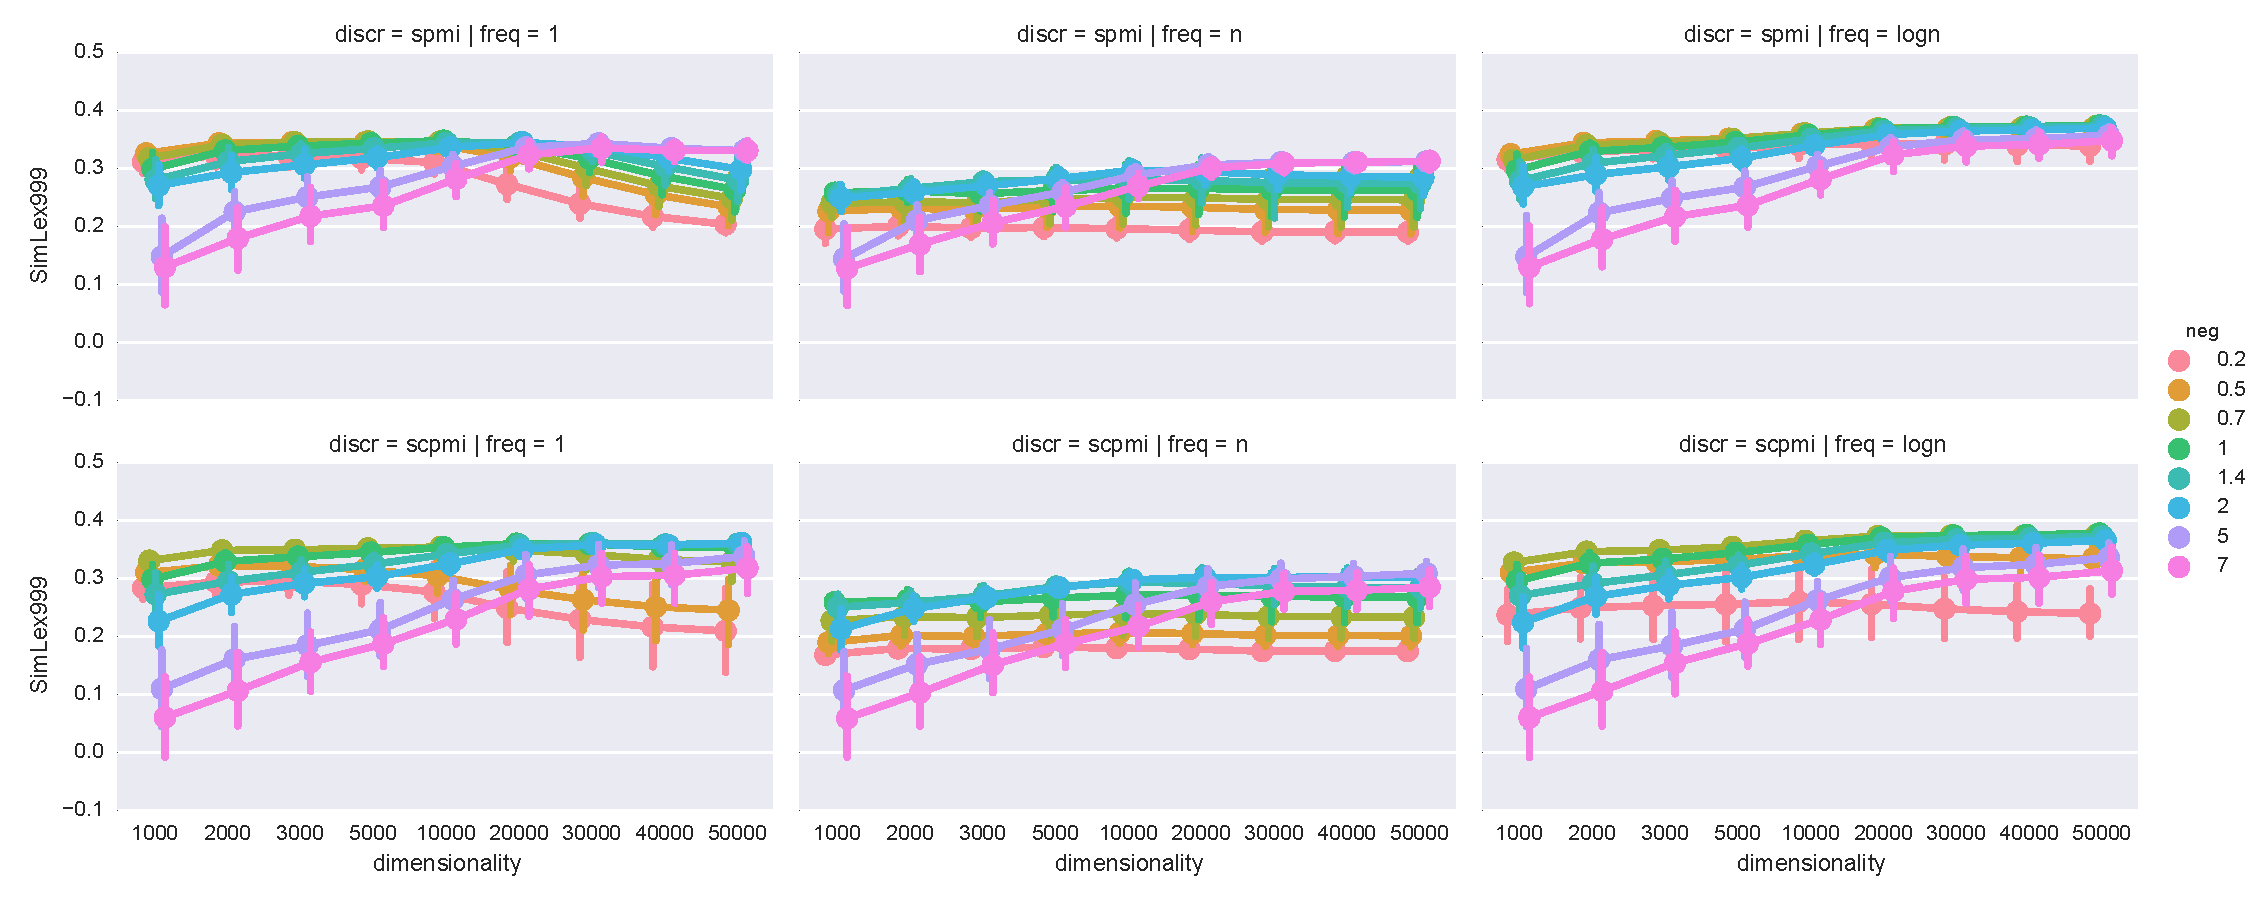
\includegraphics[width=1.11\textwidth]{supplement/figures/SimLex999-interaction-neg}}
    \caption{\small \textbf{The behaviour of shifted PMI (SPMI) on SimLex-999.}}
    \label{fig:interaction-neg}
\end{figure*}

%%% Local Variables:
%%% mode: latex
%%% TeX-master: "paper"
%%% End:


\section{Experimental setup}
\label{sec:lexical-experiments}

Table~\ref{tab:parameters} lists parameters and their values. As the source corpus we use the concatenation of Wackypedia and ukWaC \cite{Baroni2009} with a symmetric 5-word window \cite{milajevs-EtAl:2014:EMNLP2014}; our evaluation metric is the correlation with human judgements as is standard with SimLex \cite{hill2014simlex}. We derive our parameter selection heuristics by greedily selecting parameters (\texttt{cds}, \texttt{neg}) that lead to the highest average performance for each combination of frequency weighting, PMI variant and dimensionality $D$. Figures~\ref{fig:interaction-cds} and \ref{fig:interaction-neg} show the interaction of \texttt{cds} and \texttt{neg} with other parameters. We also vary the similarity measure (cosine and correlation  \cite{kiela-clark:2014:CVSC}), but do not report results here due to space limits.\footnotemark{}

\footnotetext{The results are available at \url{http://www.eecs.qmul.ac.uk/~dm303/aclsrw2016/}}

\section{Heuristics}

\paragraph{PMI and CPMI}

PMI should be used with global context probabilities. CPMI generally outperforms PMI, with less sensitivity to parameters; \NCPMI/ and \logNCPMI/ should be used with local context probabilities and \CPMI/ should apply context distribution smoothing with $\alpha = 0.75$.

\paragraph{SPMI}

10K dimensional \SPMI/ is the least sensitive to parameter selection. For models with $D>$~20K, context distribution smoothing should be used with $\alpha = 0.75$; for $D<$~20K, it is beneficial to use global context probabilities. Shifting also depends on the dimensionality: models with $D<$~20K should set $k = 0.7$, but higher-dimensional models should set $k = 5$. There might be a finer-grained $k$ selection criteria; however, we do not report this to avoid overfitting.

\logNSPMI/ should be used with global context probabilities for models with $D<$~20K. For higher-dimensional spaces, smoothing should be applied with $\alpha = 0.75$, as with \SPMI/. Shifting should be applied with $k = 0.5$ for models with $D<$ 20K,  and $k = 1.4$ for $D>$ 20K. In contrast to \SPMI/, which might require change of $k$ as the dimensionality increases, $k = 1.4$ is a much more robust choice for \logNSPMI/.

\NSPMI/ gives good results with local context probabilities ($\alpha = 1$). Models with $D<$~20K  should use $k = 1.4$, otherwise $k = 5$ is preferred.

\paragraph{SCPMI}

With \SCPMI/ and $D<$ 20K, global context probability should be used, with shifting set to $k = 0.7$. Otherwise, local context probability should be used with $\alpha = 0.75$ and $k = 2$.

With \NSCPMI/ and $D<$ 20K, global context probability should be used with $k = 1.4$. Otherwise, local context probability without smoothing and $k = 5$ is suggested.

For \logNSCPMI/, models with $D<$ 20K should use global context probabilities and $k = 0.7$; otherwise, local context probabilities without smoothing should be preferred with $k = 1.4$.

\begin{figure*}
  \centering
  \begin{subfigure}[t]{0.6\textwidth}
    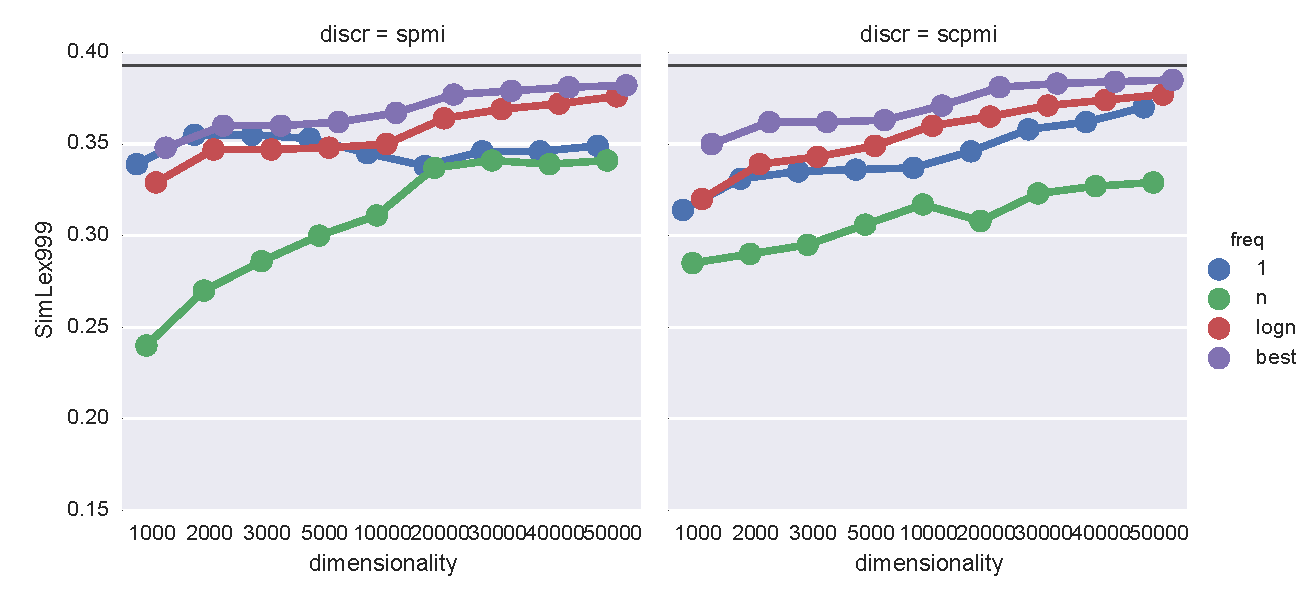
\includegraphics[width=\textwidth]{supplement/figures/SimLex999-best}
    \caption{\small \textbf{SimLex-999.}
      PPMI: 0.393,
      SVD: 0.432,
      SGNS: 0.438,
      GloVe: 0.398.
      This work: 0.385.
    }
    \label{fig:best-simlex}
  \end{subfigure}
  ~
  \begin{subfigure}[t]{0.37\textwidth}
    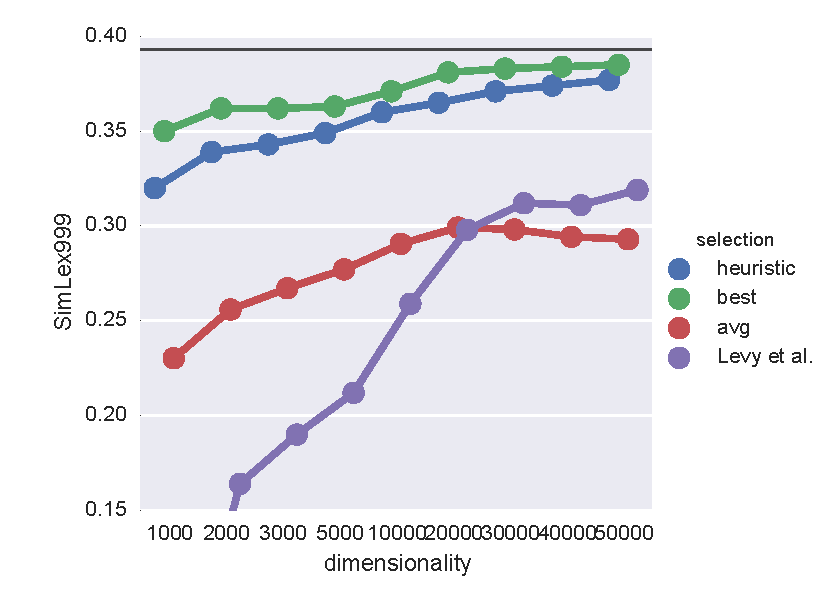
\includegraphics[width=\textwidth]{supplement/figures/SimLex999-global-best}
    \caption{}
    \label{fig:global-best-simlex}
  \end{subfigure}

  \begin{subfigure}[t]{0.6\textwidth}
    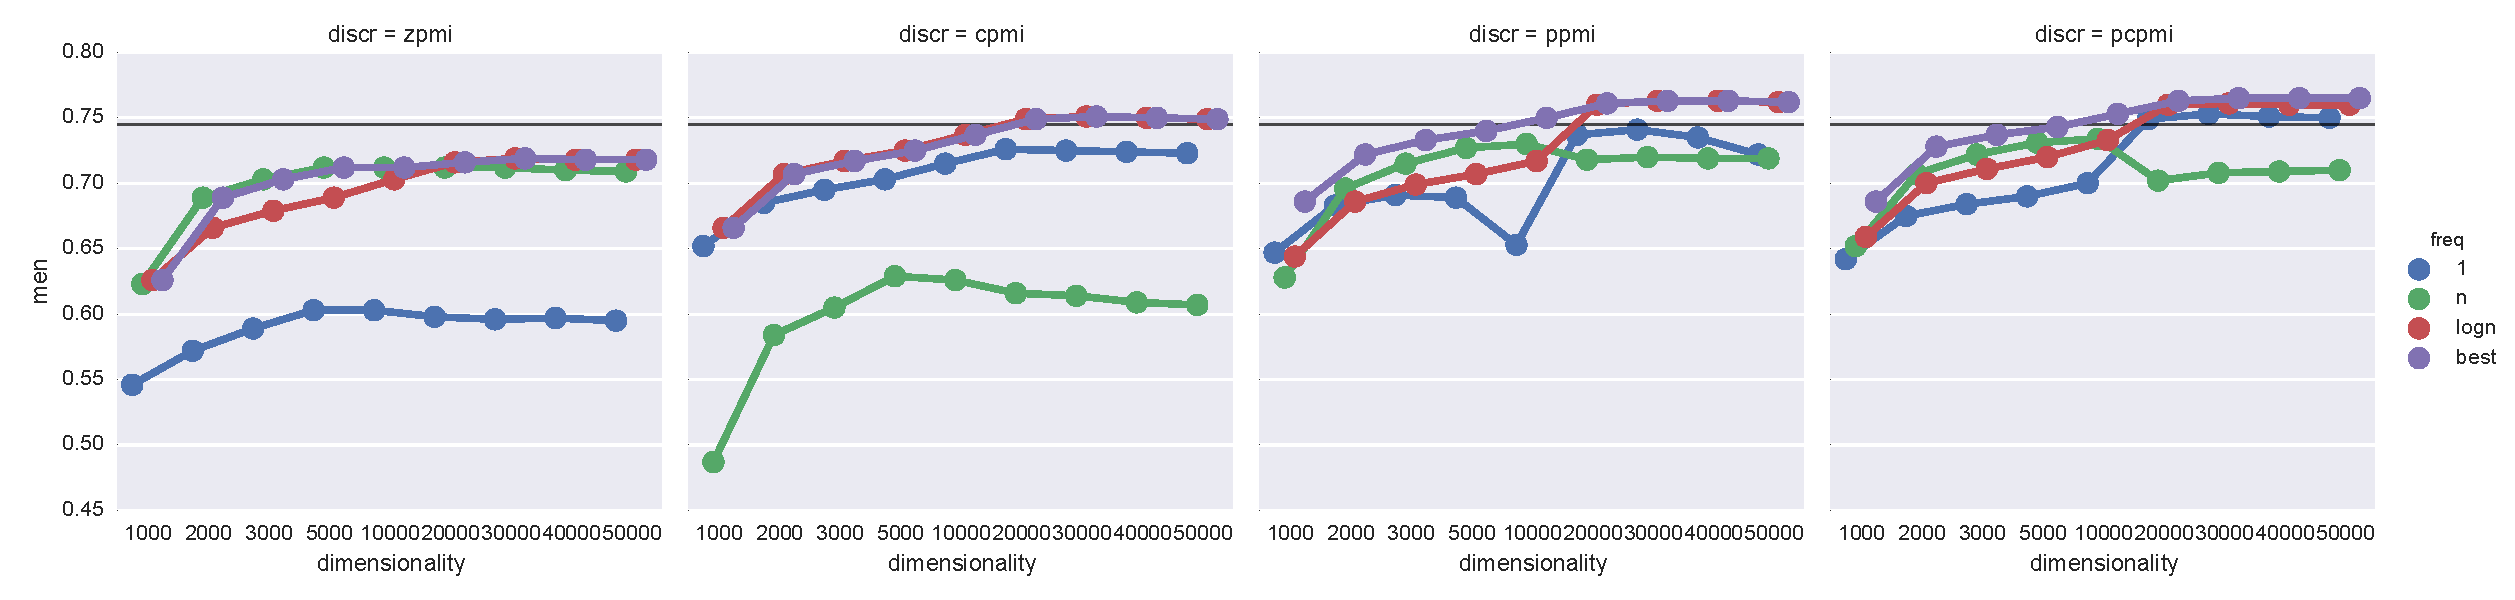
\includegraphics[width=\textwidth]{supplement/figures/men-best}
    \caption{\small \textbf{MEN.}
      PPMI: 0.745,
      SVD: 0.778,
      SGNS: 0.774,
      GloVe: 0.729.
      This work: 0.765.
    }
    \label{fig:best-men}
  \end{subfigure}
  ~
  \begin{subfigure}[t]{0.37\textwidth}
    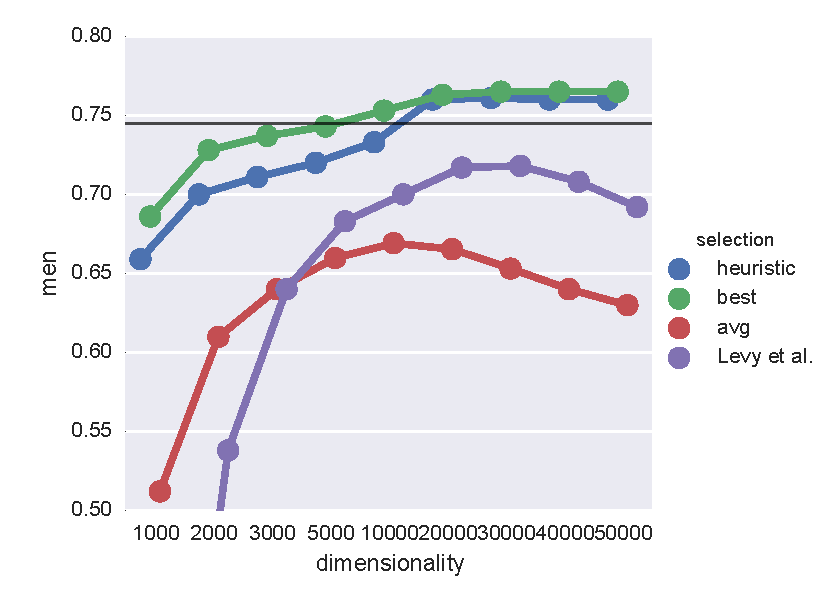
\includegraphics[width=\textwidth]{supplement/figures/men-global-best}
    \caption{}
    \label{fig:global-best-men}
  \end{subfigure}

  \caption{\small\textbf{Best configurations.} The black lines show the best count models (PPMI) reported by \protect\newcite{TACL570}. We also give our best score, SVD, SGNS and GloVe numbers from that study for comparison. On the right, our heuristic in comparison to the best and average results together with the models selected using the recommendations presented in \protect\newcite{TACL570}.}
  \label{fig:best}
\end{figure*}

%%% Local Variables:
%%% mode: latex
%%% TeX-master: "paper"
%%% End:


\section{Evaluation of heuristics}
\label{sec:heuristic-evaluation}

We evaluate these heuristics by comparing the performance they give on SimLex-999 against that obtained using the best possible parameter selections (determined via an exhaustive search at each dimensionality setting). We also compare them to the best scores reported by \newcite{TACL570} for their model (PMI and SVD), word2vec-SGNS \cite{mikolov2013efficient} and GloVe \cite{pennington2014glove}---see Figure~\ref{fig:best-simlex}, where only the better-performing SPMI and SCPMI are shown.

For \logNPMI/ and \logNCPMI/, our heuristics pick the best possible models. For \logNSPMI/, where performance variance is low, the heuristics do well, giving a performance of no more than 0.01 points below the best configuration. For \SPMI/ and \NSPMI/ the difference is higher. With \logNSCPMI/ and \SCPMI/, the heuristics follow the best selection, but with a wider gap than the SPMI models. In general $n$-weighted models do not perform as well as others.

Overall, $\log n$ weighting should be used with PMI, CPMI and SCPMI. High-dimensional SPMI models show the same behaviour, but if $D<$ 10K, no weighting should be applied. SPMI and SCPMI should be preferred over CPMI and PMI. As Figure~\ref{fig:global-best-simlex} shows, our heuristics give performance close to the optimum for any dimensionality, with a large improvement over both an average parameter setting and the parameters suggested by \newcite{TACL570} in a high-dimensional setting.\footnote{Our results using \newcite{TACL570}'s parameters differ slightly from theirs due to different window sizes (5 vs 2).}

Finally, to see whether the heuristics transfer robustly, we repeat this comparison on the MEN dataset (see Figures~\ref{fig:best-men}, \ref{fig:global-best-men}). Again, PMI and CPMI follow the best possible setup, with SPMI and SCPMI showing only a slight drop below ideal performance; and again, the heuristic settings give performance close to the optimum, and significantly higher than average or standard parameters.

\section{Conclusion}
\label{sec:conclusion}

This paper presents a systematic study of co-occurrence quantification focusing on the selection of parameters presented in \newcite{TACL570}. We replicate their recommendation for high-dimensional vector spaces, and show that with appropriate parameter selection it is possible to achieve comparable performance with spaces of dimensionality of 1K to 50K, and propose a set of model selection heuristics that maximizes performance. We foresee the results of the paper are generalisable to other experiments, since model selection was performed on a similarity dataset, and was additionally tested on a relatedness dataset.

In general, model performance depends on vector dimensionality (the best setup with 50K dimensions is better than the best setup with 1K dimensions by 0.03 on SimLex-999). Spaces with a few thousand dimensions benefit from being dense and unsmoothed  ($k < 1$, global context probability); while high-dimensional spaces are better sparse and smooth  ($k > 1$, $\alpha = 0.75$). However, for unweighted and $n$-weighted models, these heuristics do not guarantee the best possible result because of the high variance of the corresponding scores. Based on this we suggest to use \logNSPMI/ or \logNSCPMI/ with dimensionality of at least 20K to ensure good performance on lexical tasks.

\begin{table}
  \centering
  \begin{tabular}{lll}
    \toprule
    Model           & SimLex-999 & MEN \\
    \midrule
    PPMI$^*$        & 0.393      & 0.745 \\
    SVD$^*$         & 0.432      & 0.778 \\
    SGNS$^*$        & 0.438      & 0.774 \\
    GloVe$^*$       & 0.398      & 0.729 \\
    \addlinespace
    This work       & 0.385      & 0.765 \\
    \bottomrule
  \end{tabular}
  \caption{\textbf{Our model in comparison to the previous work.} On the similarity dataset our model is 0.008 points behind a PPMI model, however on the relatedness dataset 0.020 points above. Note the difference in dimensionality, source corpora and window size. SVD, SGNS and GloVe numbers are given for comparison. $^*$Results reported by \newcite{TACL570}.}
\label{tab:results}
\end{table}

There are several directions for the future work. Our experiments show that models with a few thousand dimensions are competitive with more dimensional models, see Figure~\ref{fig:best}. Moreover, for these models, unsmoothed probabilities give the best result. It might be the case that due to the large size of the corpus used, the probability estimates for the most frequent words are reliable without smoothing. More experiments need to be done to see whether this holds for smaller corpora.

The similarity datasets are transferred to other languages \cite{DBLP:journals/corr/LeviantR15}. The future work might investigate whether our results hold for languages other than English.

The qualitative influence of the parameters should be studied in depth with extensive error analysis on how parameter selection changes similarity judgements.

\section*{Acknowledgements}

We thank Ann Copestake for her valuable comments as part of the ACL SRW mentorship program and the anonymous reviewers for their comments. Support from EPSRC grant EP/J002607/1 is gratefully acknowledged by Dmitrijs Milajevs and Mehrnoosh Sadrzadeh.
Matthew Purver is partly supported by ConCreTe: the project ConCreTe acknowledges the financial support of the Future and Emerging Technologies (FET) programme within the Seventh Framework Programme for Research of the European Commission, under FET grant number 611733.

\bibliographystyle{acl2016}
\balance
\bibliography{references,dmilajevs_publications}

\end{document}
